

\chapter{Nombres complexes}

\label{chapter:Fr_01-Complex}



Pour faire court, on pourrait dire que l'algèbre est l'étude des solutions d'équations polynomiales.
Par exemple, l'algèbre \emph{linéaire} est une branche de l'algèbre qui se consacre à l'étude des solutions d'équations \emph{linéaires}. (Cette branche de l'algèbre est particulièrement intéressante lorsque l'on utilise de nombreuses variables et équations, ce que nous ferons dans le Chapitre~\href{chapter:11-solvingsystems}).



Dans le chapitre d'aujourd'hui, intéressons-nous à une conséquence fameuse de l'algèbre pour se \og remettre en jambes \fg~après un long été de vacances : les nombres complexes. C'est un incontournable pour nos chers ingénieurs (particulièrement en génie électrique) et nos chers physiciens qui vont très bientôt les utiliser à longueur de journée.


\section{Définition des nombres complexes}

L'histoire des nombres complexes est très intéressante. Elle ne commence pas comme on pourrait le croire avec la fameuse équation
$$
x^2 + 1 = 0,
$$ mais plutôt avec des équations cubiques (qui font intervenir des termes en $x^3$) !
À l'époque, tout le monde était certain que  l'équation $ x^2 + 1 = 0$
n'a pas de solution---il suffit de regarder le graphe de la fonction $y=x^2+1$ et de voir qu'il ne croise pas l'axe des abscisses. \footnote{De même, encore avant, on aurait dit que l'équation $x+1=0$ n'a pas de solution non plus puisque les nombres négatifs ne représentent pas une quantité mesurable dans la vie de tous les jours et que donc ils « n'existaient pas ».} Cependant, en se basant sur la remarque que chaque équation \emph{cubique} avec coefficients réels admet au moins une solution réelle, les nombres imaginaires (aussi longtemps appelés « nombres sophistiqués » par le mathématicien Jérôme Cardan) ont été introduits pour obtenir une formule décrivant ces solutions réelles.\footnote{Pour plus de détails, cherchez sur le web « histoire des nombres complexes ».} 


Ceci étant dit, revenons à la notation de $i$ comme étant une solution de l'équation $  x^2 + 1 = 0$;  « i » pour « imaginaire » (notation due à Euler, 1777). Alors :
\[ i^2 = -1 \qquad \text{ou bien} \qquad i = \sqrt{-1}, \]
et avec ceci nous définissons la racine carrée d'un nombre réel \emph{négatif} $a$ par
$$\sqrt{a}:=(\sqrt{\vert a\vert}) i.$$

Cela peut sembler fastidieux! En fait, si nous appliquons les règles de l'algèbre, comme dans
$$
\sqrt{-9} = \sqrt{9 \cdot (-1)} = \sqrt{9} \cdot \sqrt{-1} = 3i,
$$ nous obtenons la bonne réponse, $\sqrt{-9}=3i$, mais il faut faire très attention à la troisième égalité.
\footnote{Un vrai cours d'analyse complexe est nécessaire ici car sinon on peut avoir des problèmes, comme par exemple la contradiction $9=\sqrt{81}=\sqrt{(-9)(-9)}\not=\sqrt{ -9 }\  \sqrt{ -9 }=3i\, 3i =-9$... En effet, la règle pour les nombres réels positifs $a,\  b$ qui énonce (correctement) que : $\sqrt{ab}=\sqrt{a}\,\sqrt{b}$ \emph{n'est pas valable} en général pour les réels négatifs. Ceci peut sembler être une nuisance, mais c'est en fait la source de beaucoup de découvertes mathématiques intéressantes. Cherchez sur le web « surface de Riemann et racine carrée ».}  Contentez-vous de cette définition fastidieuse pour le moment!

(Toutefois, veuillez noter que comme en arithmétique, nous adhérons à la convention $\sqrt{a^2} =\vert a \vert$ peu importe si $a$ est positif ou négatif. En d'autres termes, quand on calcule la racine carré $\sqrt{b}$ d'un nombre réel positif $b$, la réponse à donner est l'unique
valeur positive $c$ telle que $c^2=b$, même si on aurait pu aussi prendre $c$ négative.)



Cependant, le nouveau nombre $i$ en tant que tel n'est pas tout à fait suffisant! Il va falloir qu'on puisse multiplier $i$ avec un nombre réel et y ajouter un nombre réel. En effet par exemple, considérons l'équation
$$
x^2 + 4x + 8 = 0.
$$
Par la formule quadratique, cette équation donne les deux racines suivantes :
$$
x = \frac{-4 \pm \sqrt{16-32}}{2} = -2 \pm \frac12 \sqrt{-16} = -2 \pm \frac12 (4i) = -2 \pm 2i,
$$
où nous avons simplifié $\sqrt{-16}$ grâce à la définition « fastidieuse » introduite précédemment.
Vérifions que ces racines ont bien un sens. Substituons d'abord $x = (-2+2i)$ dans l'équation quadratique et simplifions :
$$
(-2+2i)^2 + 4(-2+2i) + 8 = (4 -4i - 4i + 4i^2) + (-8 +8i) +8 = 4+4i^2 = 0\,,
$$
où dans la dernière étape nous appliquons $i^2 = -1$. On obtient donc bien $0$. De même, nous
pouvons vérifier que $-2-2i$ est aussi racine de l'équation.




Ayant cette remarque à l'esprit ainsi que la formule quadratique
, nous arrivons à la définition suivante.

\begin{definition}
L'ensemble des \emph{nombres complexes} est l'ensemble
$$
\C = \{ a+b\,i \colon a, b \in \mathbb{R} \}.
$$
\noindent(\`A interpréter comme:  « l'ensemble de tous les objets de la forme $a+bi$, où $a$ et
$b$ sont des nombres réels »).

Lorsque l'on écrit
$$
z =a +b\,i \in \C,
$$
on veut dire  $z$ (ou $a+b\,i $) appartient à $\C $.\\
\indent Terminologie:
$a$ est appelé la \emph{partie réelle} de $z$ (notée $Re(z)$) et $b$ est appelé
la partie imaginaire de $z$ (notée $Im(z)$).  Notez que $Re(z)$ et $Im(z)$ sont des nombres \emph{réels} !


Lorsque $Re(z)=0$, alors $z=bi $ et nous dirons que $z $ est un \emph{imaginaire pur}; et
quand $Im(z)=0$, alors $z=a$ et on dit que $z$ est un \emph{réel pur}.  Ainsi $\R \subset \C$, ce qui se lit :  $\R$
est un sous-ensemble de $\C$.

\end{definition}

De même que les nombres réels sont représentés sur une droite, la droite des nombres réels, les nombres complexes sont représentés dans un plan, 
le \emph{plan complexe}, que nous étudierons bientôt.

Rappelez-vous bien que, pour toute équation quadratique $ax^2+bx+c=0$ dont les coefficients $a,\, b,\, c$ sont réels, les racines sont de la forme $$x = \frac{-b}{2a} \pm \frac{\sqrt{b^2-4ac}}{2a}. $$ Si $b^2-4ac \geq 0$, les racines sont (purement) réelles. Sinon, elles sont des nombres complexes.  Donc au final, TOUTES les équations quadratiques admettent DEUX racines (en adoptant la convention qu'une racine double est comptée comme deux racines à partir de maintenant).

\section{Algèbre des nombres complexes}

\begin{itemize}
\item Égalité: $a+bi = c+di \Leftrightarrow\,  a=c\, \textrm{ et }\, b=d$.
\item Addition : $(a+bi) + (c+di) = (a+c) + (b+d)i$.
\item Multiplication : $(a+bi)(c+di) = (ac-bd) + (ad+bc)i$.
\end{itemize}

En fait, les nombres complexes satisfont les mêmes propriétés 
que les nombres réels, sauf qu'il n'y a pas de relation d'ordre (c'est-à-dire que l'expression « $z>y$ » n'a pas de sens avec les nombres complexes).

{\bf Question:} Qu'en est-il de la division ?

\begin{myexample}
Essayons de résoudre l'équation $(4+3i)z = 1$, si possible. Autrement dit, qu'entendons-nous par la fraction suivante : 
$$
z = \frac{1}{4+3i} \,?
$$
(SVP SVP rappelez-vous que par exemple $\frac{1}{2+3} \neq \frac12 + \frac13$ !!!)


\begin{mysol}
Idée : rappelez-vous que $i$ est une racine carrée puis utilisez le processus standard de l'algèbre appelée \emph{rationalisation du dénominateur}.

Remarquez que
 $$(a+b \, i)(a-b\, i) = a^2-(b\, i)^2 = a^2+b^2,$$ et comme $a$ et $b$ sont \emph{réels}, on a $a^2+ b^2 \neq 0$
sauf si $a$ et $b$ sont tous les deux nuls.

En considérant le nombre complexe $z=a+bi$ avec $a,\, b\in\R$, on définit :
\begin{itemize}
\item $\overline{z} = a-bi$ s'appelle le \emph{conjugué} (complexe) de $z$. Notez que nous avons en fait déjà utilisé des conjugués complexes dans la formule quadratique. Essentiellement, l'idée pour calculer $\overline{z}$ à partir de $z$ est de remplacer « $ i $ » par « $ -i $ », et il n'est même pas nécessaire d'avoir simplifié l'expression de $z$ au préalable avant de faire un tel remplacement.
\item $| z | = \sqrt{a^2+b^2}$ s'appelle le \emph{module} de $z$. Contrairement à $z$ qui est un nombre complexe, son module $|z|$ est un nombre réel.
\item La forme $z=a+bi$, où $a,\, b\in\R$, s'appelle la \emph{forme cartésienne} de $z$. On verra plus tard d'autres formes pour écrire un nombre complexe.
\end{itemize}

Soulignons que l'égalité
$z = 0$ est vraie si et seulement si (ssi) $\vert z \vert = 0$, et contrairement aux nombres complexes, nous POUVONS toujours
comparer le module des nombres complexes : par exemple $\vert i \vert =  1 > 0 =  \vert 0 \vert$; ceci est vrai car, comme on l'a dit, le module $|z|$ est toujours un nombre réel.

Maintenant que nous avons rappelé les notions de conjugué et de module d'un nombre complexe, on peut s'intéresser à l'expression suivante :
$$
z \overline{z} = \vert z \vert^2 = \vert \overline{z} \vert^2,
$$
laquelle donne
$$
z \cdot \left(\frac{\overline{z}}{\vert z \vert^2}\right) = 1
$$
ou encore
$$
\frac{1}{z} = \frac{\overline{z}}{\vert z \vert^2}.
$$

Ainsi, dans notre exemple, on obtient finalement :
$$
\frac{1}{4+3i} = \left(\frac{1}{4+3i} \right) \left( \frac{4-3i}{4-3i} \right) = \frac{4-3i}{4^2+3^2} = \frac{4-3i}{25} = \frac{4}{25} - \frac{3}{25}i.
$$
\end{mysol}
\end{myexample}

\begin{myprob}
Écrire sous forme cartésienne $a+b\,i$ le nombre complexe suivant :
$$
\frac{3+2i}{-2+4i}\, .
$$

\begin{mysol}
Multipliez par $1 = \frac{-2-4i}{-2-4i}$ puis simplifiez comme suit :
$$
\frac{3+2i}{-2 + 4i} = \frac{3+2i}{-2 + 4i}\cdot \frac{-2-4i}{-2-4i} =
\frac{(3+2i)(-2-4i)}{4+8i-8i-16i^2} = \frac{2-16i}{20} = \frac{1}{10} - \frac{4}{5}i.
$$
Ainsi, il suffit de prendre $a=\frac{1}{10}$ et $b=-\frac45$.
\end{mysol}
\end{myprob}

Voici d'autres propriétés faciles à démontrer.

\begin{lemma}[Propriétés des nombres complexes]
 Pour
$z,w \in \C$ et $c\in \R$, on a:
\begin{enumerate}
\item $\frac{1}{z} = \frac{\overline{z}}{\vert z \vert^2}$;\smallskip
\item $\overline{z+w} = \overline{z} + \overline{w}$;
\item $\overline{cz} = c\overline{z}$;
\item $\overline{zw} =\overline{z}\; \overline{w}$;
\item $\overline{z/w} = \overline{z}/\overline{w}$.\smallskip
\item $\overline{\overline{z}} = z$  (e.g. : $\overline{\overline{3+2i}}= \overline{3-2i} = 3+2i$);
\item $\overline{z} = z$ ssi $z \in \R$;
\item $\overline{z} = -z$ ssi $z$ est un imaginaire pur;
\item $\vert z \vert  \in \R$ et $\vert z \vert \geq 0$;
\item $\vert z \vert = \vert \overline{z} \vert$;
\item $\vert zw \vert = \vert z \vert \, \vert w \vert$;
\item $\vert z/w \vert = \vert z \vert / \vert w \vert$;
\item $\vert z + w \vert \leq \vert z \vert + \vert w \vert$ (« Inégalité triangulaire »);
\item Si $a$ est un nombre réel, alors $\vert a + 0i \vert$ est la valeur absolue de $a$.
  (On écrit simplement $z=a$ plutôt que $z=a+0i$).
\end{enumerate}


\end{lemma}

\begin{proof}
Nous prouvons ici deux de ces propriétés et nous laissons les autres en exercice aux soins du lecteur.
(Conseils : pour l'inégalité triangulaire, une astuce est d'utiliser la géométrie des nombres complexes, cf. section 1.3. Pour les propriétés avec des multiplications de nombres complexes, il est plus simple d'utiliser la forme polaire, cf. sections 1.4 et 1.5).

\begin{enumerate}
	\item[2.] Supposons que $z$ et $w$ sont des nombres complexes.
Alors $z$ s'écrit
$z = a+bi$ pour certains nombres réels $a$ et $b$, et $w = c+di$
pour certains nombres réels $c$ et $d$.

D'une part, on a $z+w = (a+c) + (b+d)i$ et donc $$\overline{z+w} = (a+c) - (b+d)i.$$

D'autre part, on a $\overline{z} = a-bi$ et $\overline{w} = c-di$, ce qui donne
$$\overline{z} + \overline{w} = (a+c)+(-b-d)i = (a+c)-(b+d)i.$$

Les deux côtés sont donc égaux, ce qui complète la preuve.


	\item[10.] Supposons que $z$ est un nombre complexe.  Comme
$
\vert z \vert = \sqrt{z \overline{z}},
$
on a
$$
\vert \overline{z} \vert = \sqrt{\overline{z} \ \overline{\overline{z}}}  = \sqrt{\overline{z} z }= \sqrt{ z \overline{z} }= \vert z \vert.
$$
CQFD.
\end{enumerate}
\end{proof}


\section{Géométrie des nombres complexes}

\begin{center}
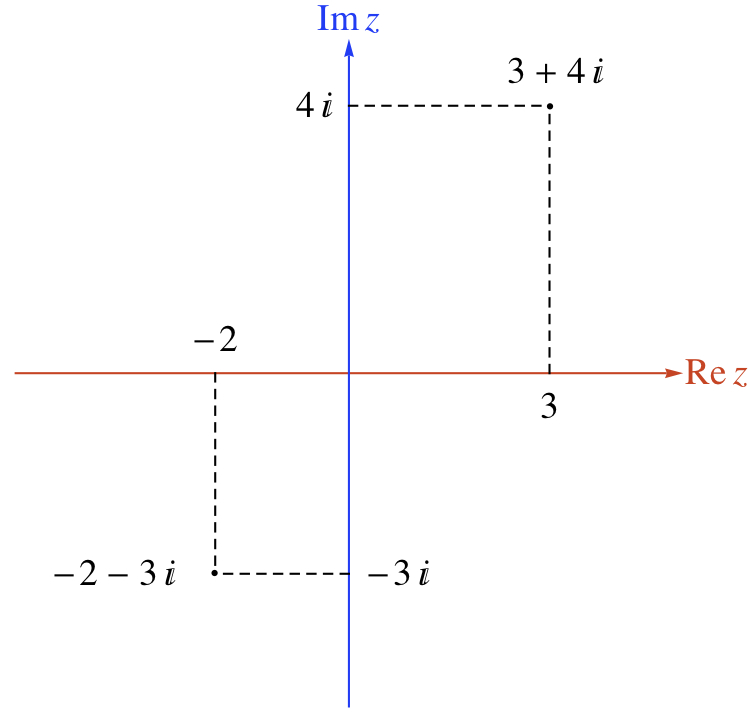
\includegraphics[scale=.4]{complexplane.jpg}~\\[1cm]
\end{center}
Chaque nombre complexe $z$
peut s'écrire de manière unique sous la forme $z=a+b\,i$ pour certains nombres réels $a$ et $b$. Pour représenter $z$ dans un graphique,
on lui associe le point de coordonnées $(a,b)$ dans le plan $xy$.
Ainsi $z=a+b\,i$ est vu comme un point du plan $xy$, et nous appellerons donc ce plan le \emph{plan complexe}.  L'axe horizontal est appelé
l'\emph{axe réel} et l'axe vertical
est appelé l'\emph{axe imaginaire}.



L'addition de deux nombres complexes est la même que l'addition de
deux vecteurs dans le plan.  L'opposé $-z$ d'un nombre complexe $z$ correspond au vecteur opposé du vecteur lié à $z$, comme représenté sur le dessin ci-dessus.  La multiplication
par un nombre réel est simplement la multiplication scalaire d'un vecteur, mais la multiplication
par un nombre complexe est plus subtile : c'est en fait une combinaison de rotation et d'homothétie.
(Essayez de faire les calculs pour voir ce que ça donne !)

Le conjugué complexe $\overline{z}$ correspond juste la symétrie par rapport à l'axe réel.  Ainsi, les nombres complexes $z = a+b\,i$ et $\overline{z} = a-b\,i$ ont la même abscisse mais leurs ordonnées sont opposées.

Le module $|z|$ de $z$ est simplement la longueur du vecteur représentant $z$.
(Rappelons que la formule de la longueur du vecteur de coordonnées $(a,b)$ est simplement
$\sqrt{a^2+b^2}$. )

\section{Forme polaire d'un nombre complexe}


Dans cette section nous ré-écrirons les nombres complexes sous une nouvelle forme, la \emph{forme polaire} $z= r\, e^{i\, \theta}$. Notez que les coordonnées $(r,\theta)$ sont aussi appelées « coordonnées polaires » dans le cas du plan réel $\mathbb R^2$, cf. les cours Calcul II et Calcul III.


 \begin{center}
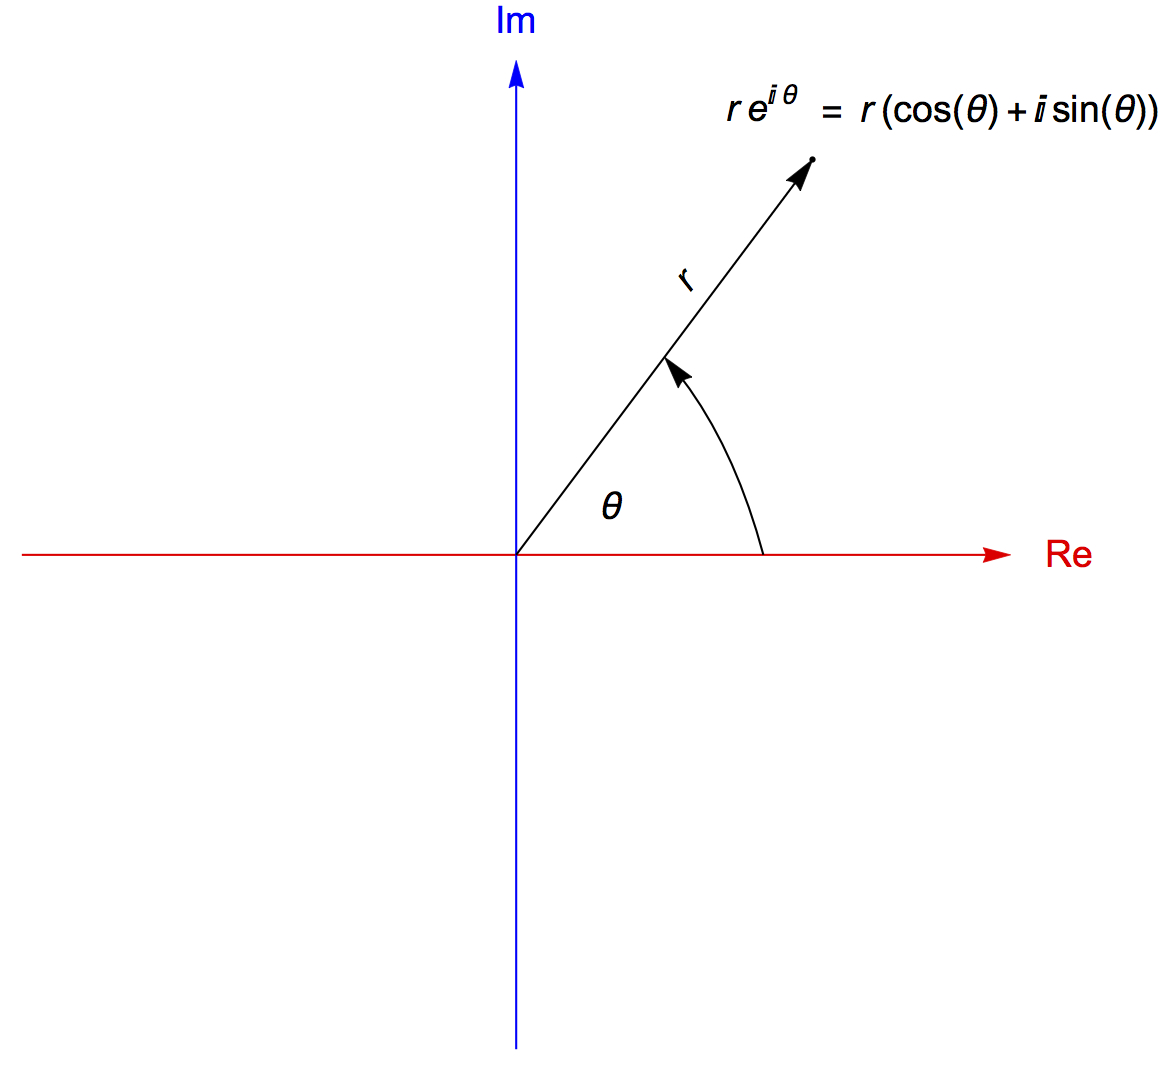
\includegraphics[scale=.4]{PolarForm.jpg}~\\[1cm]
\end{center}




Si $z = x+y\,i \in \C$ est non-nul, alors on définit 
$$
r = \vert z \vert = \sqrt{x^2+y^2} \neq 0,
$$
et par les formules trigonométriques, on a :
$$
\frac{x}{r} = \cos(\theta), \qquad \frac{y}{r} = \sin(\theta).
$$
Par conséquent, on peut écrire
$$
z = x+yi = r \cos(\theta) + i r\sin(\theta) = r(\cos(\theta)+i \sin(\theta)).
$$

L'angle $\theta$ est noté $\theta = arg(z)$ et s'appelle \emph{argument} de $z$. Remarquez que $\theta$ n'est pas déterminé de fa\c{c}on unique
puisque n'importe quel $\theta' = \theta + 2n\pi$ avec $n\in \Z$ fonctionne aussi.  C'est pour cela qu'en général nous
choisirons $\theta$ tel que $-\pi < \theta \leq \pi$, qui lui par contre est unique, que nous noterons $\theta = Arg(z)$ et que nous appellerons l'\emph{argument principal} de $z$.

En 1748, Euler a démontré que

$$
e^z = 1 + z + \frac{z^2}{2} + \cdots = \sum_{n=0}^\infty \frac{z^n}{n!}.
$$
(C'est ce qu'on appelle généralement \emph{série entière}). De manière surprenante, en comparant les séries entières avec les fonctions trigonométriques,
on obtient la formule élégante :
$$
e^{i\theta} = \cos(\theta) + i\sin(\theta).
$$
La notation moderne de la \emph{forme polaire} du nombre complexe $z$ est donc simplement :
$$
z = r \,e^{i\theta}.
$$

\begin{myexample} \label{ex: calculer quelques formes polaires}
À partir du diagramme ci-dessous, vérifiez que $2i= 2\,e^{i \frac{\pi}2}$, $-i=e^{-i \frac{\pi}2}$, $-1 = e^{i\pi}$ et
$1+i =\sqrt{2}\,e^{i \frac{\pi}4}$.
\end{myexample}
\begin{center}
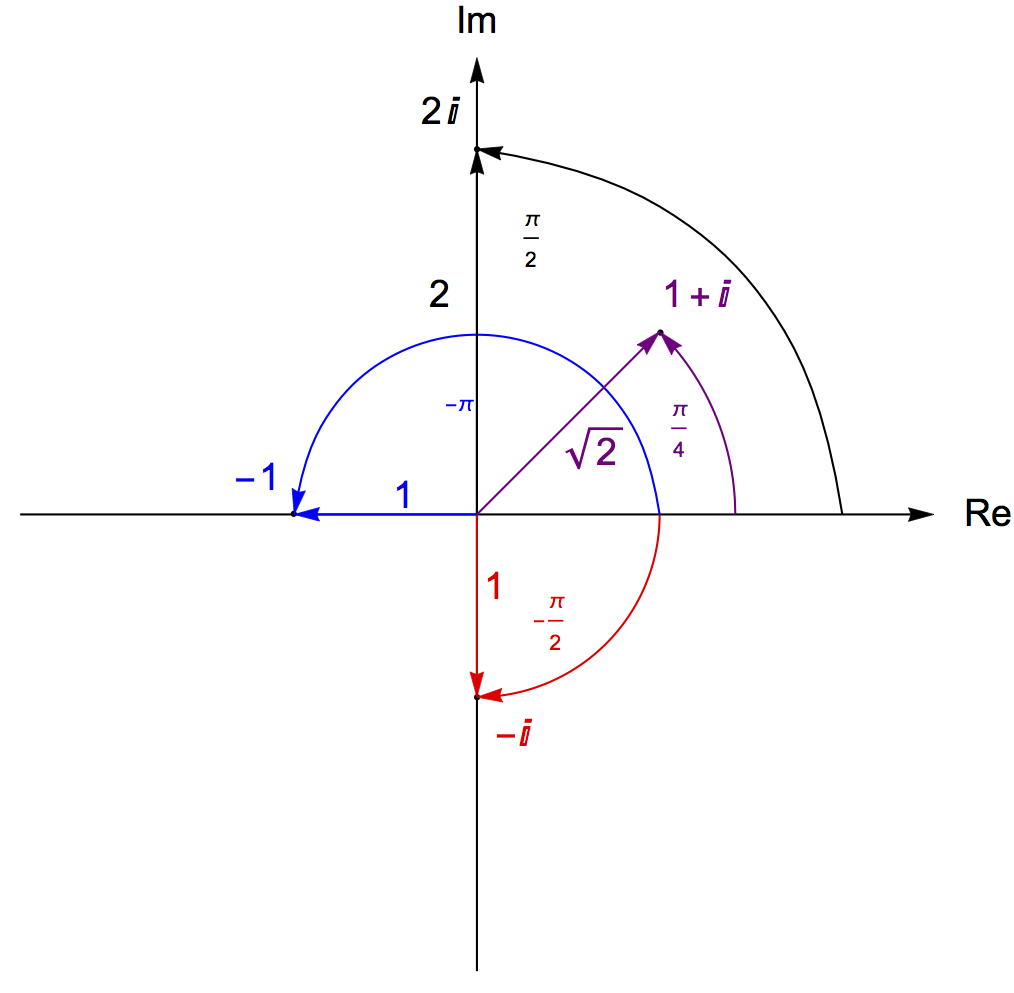
\includegraphics[scale=.4]{PolarFormExample.jpg}~\\[1cm]
\end{center}


Notez que nous avons également les propriétés suivantes :
\begin{itemize}
\item $re^{i\theta} = r' e^{i\theta'}$ ssi $r=r'$ et $\theta = \theta' + 2n\pi$ pour un certain $n\in \Z$;
\item $\overline{re^{i\theta}} = re^{-i\theta}$;
\item $\vert e^{i\theta} \vert = 1$ pour tout $\theta\in\R$.
\end{itemize}

\section{Multiplication de nombres complexes sous forme polaire}

Soient $z = re^{i\theta}$ et $w = se^{i\phi}$. Alors
\begin{align*}
zw &= \left( r(\cos(\theta)+i\sin(\theta)) \right) \left(s (\cos(\phi)+i\sin(\phi)\right) \\
&= (rs)\left( (\cos(\theta)\cos(\phi) - \sin(\theta)\sin(\phi)) + i(\cos(\theta)\sin(\phi) + \sin(\theta)\cos(\phi)) \right)\\
&= rs\,(\cos(\theta + \phi) + i\sin(\theta + \phi))\\
&= rs\,e^{i(\theta+\phi)}.
\end{align*}
On se retrouve donc avec la formule habituelle de la multiplication avec des exposants.  (Idem pour la
division, on retrouve la formule habituelle.)

\begin{myprob}
Écrire sous forme polaire le nombre complexe suivant : 
$$
\frac{i}{1+i}\, .
$$

\begin{mysol}
D'après l'exemple \ref{ex: calculer quelques formes polaires}, nous avons $i = e^{i\frac{\pi}{2}}$ et
$1+i = \sqrt{2}\,e^{i\frac{\pi}{4}}$.
Donc
$$
\frac{i}{1+i} = \frac{e^{i\frac{\pi}{2}}}{\sqrt{2}\,e^{i\frac{\pi}{4}}}
 = \frac{1}{\sqrt{2}}\,e^{i\frac{\pi}{4}}\, .
$$
(Vérifiez aussi ceci en utilisant la première méthode avec la forme cartésienne, et vous verrez quelle est un peu plus lente que la nouvelle méthode.)
\end{mysol}
\end{myprob}

\section{Le Théorème fondamental de l'algèbre}



Nous avons déjà vu que toute équation quadratique à coefficients réels admet deux racines complexes. Remarquez d'ailleurs que si l'une des deux racines $z$ n'est pas réelle, alors l'autre non plus n'est pas réelle car elle correspond au complexe conjugué $\overline{z}$. 

Inversement, étant donné un nombre complexe $z$, on peut toujours trouver un polynôme à coefficients réels dont les
racines sont exactement $z$ et $\overline{z}$ :
$$
(x-z)(x-\overline{z}) = x^2 -(z+\overline{z})x + z \overline{z}.
$$
Heu... mais est-ce que les coefficients de ce polynôme sont vraiment réels ?  HÉ OUI !  Écrivez
$z = a+ib$; alors $z+\overline{z} = 2a$ est réel, et
$z \overline{z} = |z|^2$ aussi comme nous l'avons prouvé précédemment.

En résumé, tout polynôme à coefficients réels admet au moins une racine complexe (lorsque bien sûr le polynôme n'est pas constant...), et tout nombre complexe est racine d'au moins un certain polynôme à coefficients réels.

Notez toutefois que si vous prenez deux nombres complexes $z$ et $w$ qui ne sont pas conjugués, alors le polynôme $(x-z)(x-w)$ n'est pas forcément à coefficients réels, il est en général à coefficients complexes...
Ceci nous amène à la question suivante : si vous prenez une équation quadratique
à coefficients complexes et que vous utilisez la formule quadratique pour
pour la résoudre, de quels nombres supplémentaires (comme $i$) aurez-vous besoin ?

Réponse : en fait, comme l'énonce le théorème suivant, AUCUN !  Les nombres complexes sont tellement généraux qu'ils englobent tout ce dont vous aurez besoin à jamais (ou du moins pour très longtemps) ! C'est ça qui fait le vrai intérêt des nombres complexes.

\begin{theorem} [Théorème fondamental de l'algèbre] \label{theoreme : theoreme fondamental de l algebre}
Tout polynôme à coefficients dans $\C$
se factorise complètement en facteurs simples de la forme $ax+b$,
avec $a,\, b \in \C$.
\end{theorem}

\section[Réflexions sur le Théorème fondamental de l'algèbre]{Quelques réflexions sur la signification du Théorème fondamental de l'algèbre}

Le théorème \ref{theoreme : theoreme fondamental de l algebre} justifie en quelque sorte l'existence des nombres complexes $\C$.
En effet, pour un algébriste, une équation quadratique devrait toujours avoir $2$ racines puisque c'est une équation avec un polynôme de degré $2$, et de même une équation cubique devrait toujours avoir $3$ racines à cause du polynôme de degré $3$. Ou même plus généralement, une équation donnée par un polynôme de degré $n$ devrait admettre $n$ racines.

Mais comme on l'a vu, la quadratique
$x^2+2$ n'a pas de racine réelle...
En effet, en Calcul,
on justifie cette remarque en tra\c{c}ant le graphe de $y=x^2+2$ et en argumentant
« Regardez, le graphe ne coupe pas l'axe des $x$. »  Cela explique tout---ou presque...
Mais pour un algébriste ceci ne répond pas à la question, et il vous dira  « il vous manque encore deux racines à trouver~»!

En algèbre, nous cherchons à unifier les thèmes en trouvant des points
communs à certains types de problèmes. Nous sommes comme à la conqu\^ete
de (merveilleuses) solutions universelles, et les nombres complexes sont
un exemple de solution universelle : après avoir ajouté $\sqrt{-1}$,
tous les problèmes ont soudain une solution, $x^2+2$ admet bien deux racines
et $ix^7+3x^2-(4+i)$ admet bien 7 racines !

(Bon, en réalité, « tous » les problèmes ne sont pas complètement résolus.
En effet, le Théorème fondamental de l'algèbre dit qu'il existe des racine, mais il ne dit RIEN sur COMMENT
TROUVER ces racines.  Il dit simplement qu'elles existent.  On finit donc toujours par
revenir au cours de Calcul pour nous aider à concrètement trouver ces racines.)

Dans le restant de ce livre, nous allons étudier l'algèbre LINÉAIRE,
une branche particulière de l'algèbre, où il s'avère qu'il existe
des solutions universelles pour absolument tous les problèmes
(non seulement «~l'existence~», mais aussi des outils pour réellement trouver ces solutions, wow !).





